\documentclass{article}

\usepackage{graphicx}
\usepackage{tikz}
\usepackage{tikzsymbols}
\usetikzlibrary{calc,patterns,shapes.geometric}
\pagestyle{empty}
\usepackage[margin=0pt]{geometry}
\geometry{papersize={14in,12in}}

\def\centerarc[#1](#2)(#3:#4:#5){\draw[#1] ($(#2)+({#5*cos(#3)},{#5*sin(#3)})$) arc (#3:#4:#5);}

\begin{document}
	\begin{figure}
		\centering
		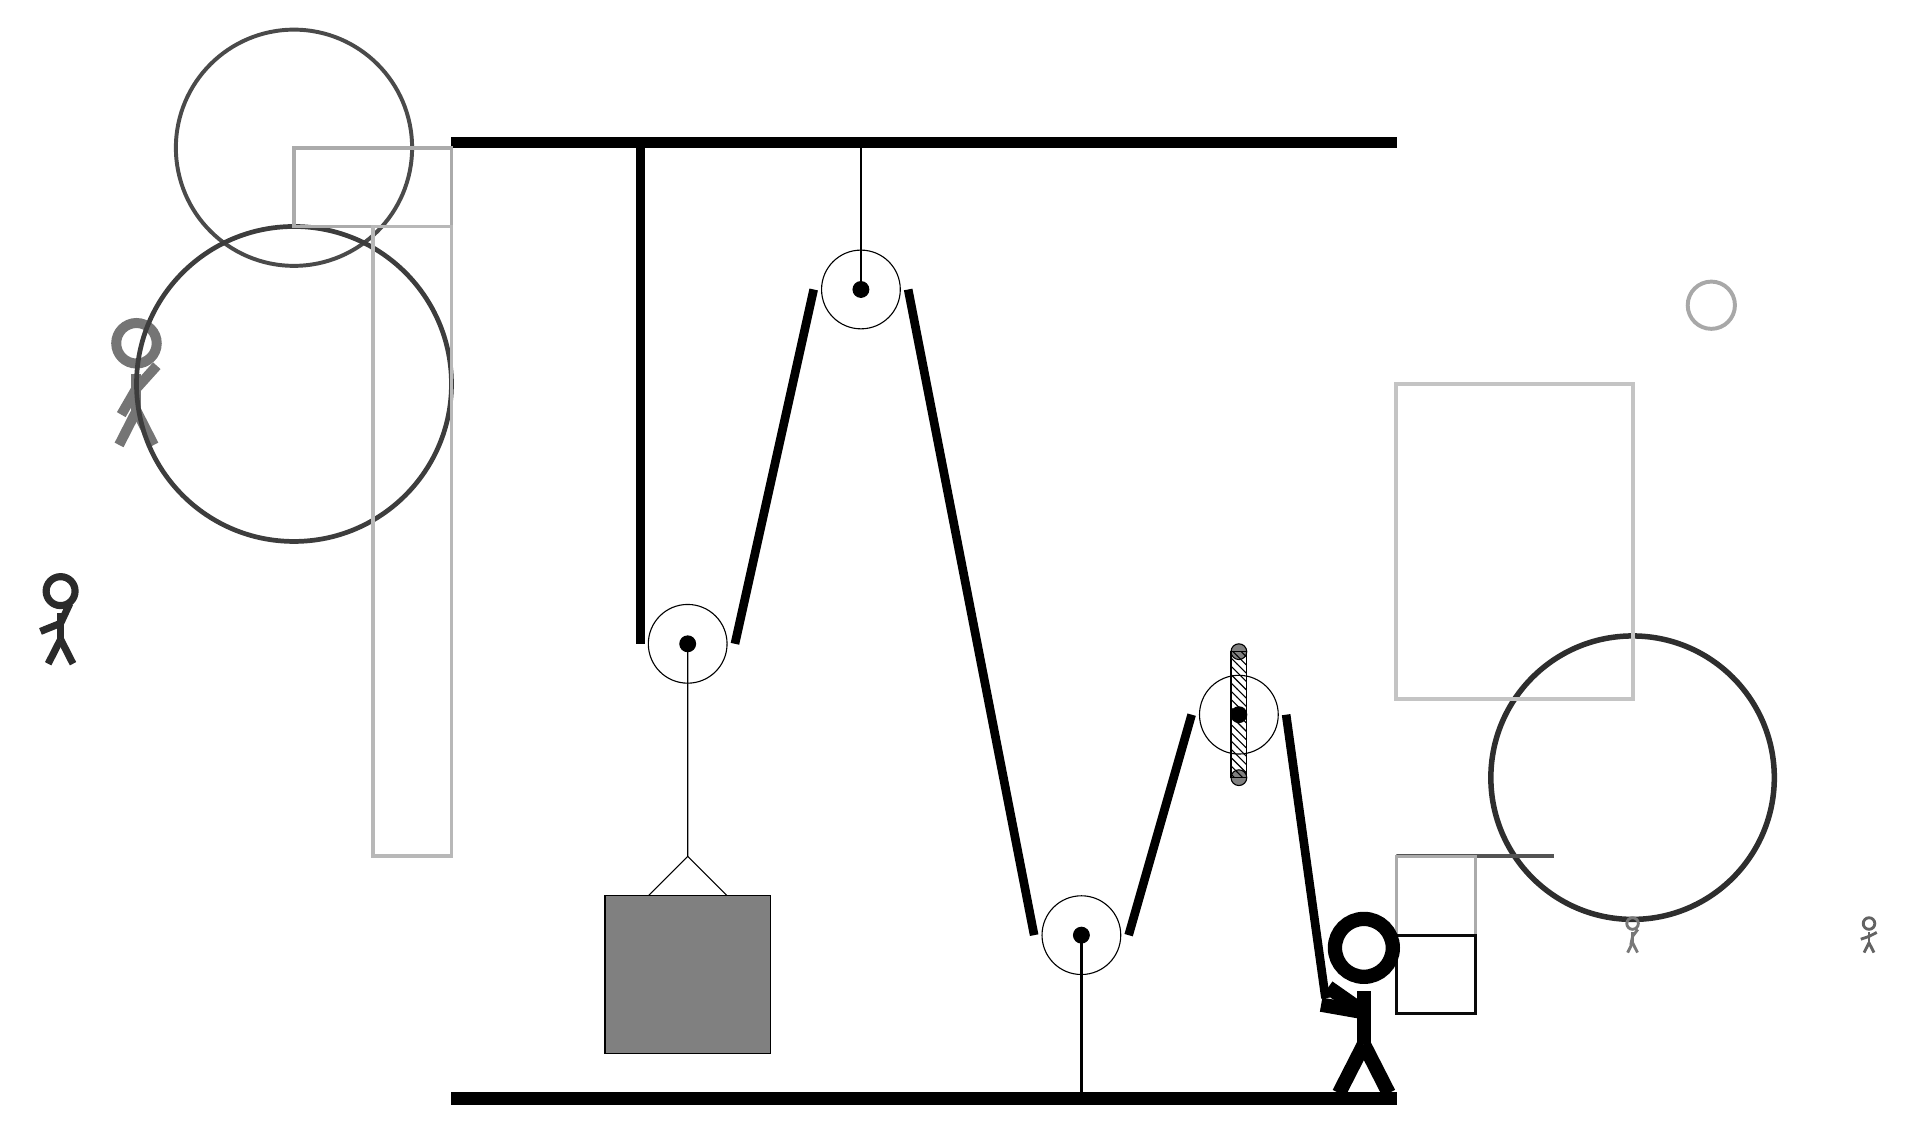
\begin{tikzpicture}
			%%%%% START %%%%%
			
			\draw[fill=black] (-2, 9) rectangle (10, 9.125);
			
			\draw (1, 2.7) circle (0.5);
			\draw[fill=black] (1, 2.7) circle (0.1);
			
			\node[line width=0.5mm, color=black!83] at (-7, 3) {\Strichmaxerl[5][22][65]};
			
			\draw [line width=0.5mm, color=black!71](-4, 9) circle (1.5);
			\node[line width=0.4mm, color=black!54] at (-6, 6) {\Strichmaxerl[7][60][48]};
			\draw [line width=0.7mm, color=black!82](13, 1) circle (1.8);
			\draw [line width=0.5mm, color=black!34](14, 7) circle (0.3);
			\draw [line width=0.6mm, color=black!76](-4, 6) circle (2.0);
			
			\draw[line width=0.5mm, color=black!67] (10, 0) rectangle (12, 0);
			\draw[line width=0.4mm, color=black!33] (11, -2) rectangle (10, 0);
			\draw[line width=0.5mm, color=black!33] (-2, 9) rectangle (-4, 8);
			\node[line width=0.6mm, color=black!61] at (16, -1) {\Strichmaxerl[2][19][27]};
			
			\draw[line width=0.5mm, color=black!23] (10, 6) rectangle (13, 2);
			\draw[line width=0.5mm, color=black!28] (-2, 0) rectangle (-3, 8);
			\node[line width=0.6mm, color=black!53] at (13, -1) {\Strichmaxerl[2][78][53]};
			
			\draw[line width=0.4mm, color=black!96] (10, -1) rectangle (11, -2);
			
			\draw (3.2, 7.2) circle (0.5);
			\draw[fill=black] (3.2, 7.2) circle (0.1);
			\draw[thick] (3.2, 7.2) -- (3.2, 9);
			
			\draw (6, -1) circle (0.5);
			\draw[fill=black] (6, -1) circle (0.1);
			\draw[thick] (6, -1) -- (6, -3);
			
			\draw[fill=white](8, 1.8) circle (0.5);
			\draw[fill=black] (8, 1.8) circle (0.1);
			\draw[fill=black!50] (8, 2.6) circle (0.1);
			\draw[fill=black!50] (8, 1.0) circle (0.1);
			\draw[pattern=north west lines, pattern color=black] (7.9, 2.6) rectangle (8.1, 1.0);
			
			\draw (1, 2.7) -- (1, 0) -- (0.5, -0.5);
			\draw (1, 0) -- (1.5, -0.5);
			\draw[fill=black!50] (-0.05, -0.5) rectangle (2.05, -2.5);
			
			\draw[line width=1.1mm] (0.4, 9) -- (0.4, 2.7);
			\centerarc[line width=1.1mm](1, 2.7)(180:360:0.6);
			\draw[line width=1.1mm](1.6, 2.7) -- (2.6, 7.2);
			\centerarc[line width=1.1mm](3.2, 7.2)(0:180:0.6);
			\draw[line width=1.1mm](3.8, 7.2) -- (5.4, -1);
			\centerarc[line width=1.1mm](6, -1)(180:360:0.6);
			\draw[line width=1.1mm](6.6, -1) -- (7.4, 1.8);
			\centerarc[line width=1.1mm](8, 1.8)(0:180:0.6);
			\draw[line width=1.1mm](8.6, 1.8) -- (9.1, -1.8);
			
			\node at (9.5, -1.9) {\Strichmaxerl[10][-35][170]};
			
			\draw[fill=black] (-2, -3) rectangle (10, -3.15);
			
			%%%%% END %%%%%
		\end{tikzpicture}
	\end{figure}	
\end{document}